\section{Modified Keplerian Hohmann Transfer}\label{sec:ModifiedHohmann}
Since the orbits of both Earth and Mars are assumed circular in this investigation, the lowest
maneuver cost transfer between the two bodies under Keplerian dynamics is a Hohmann transfer,
appearing in \cref{fig:Hohmann}. However, the Hohmann equations only apply when the orbits are
coplanar. Hence, a plane change maneuver is introduced to account for the difference in the
planetary orbital planes. Inclination change maneuvers have the lowest magnitude at apoapsis,
achieved here by including the plane change in the maneuver cost of the second Hohmann burn
($\Delta v_{2}$ in \cref{fig:Hohmann}) to form a modified Hohmann transfer that serves as the
baseline $\Delta v$ cost for Keplerian patched conic transfers between Earth and Mars.

\begin{figure}[H]
    \centering
    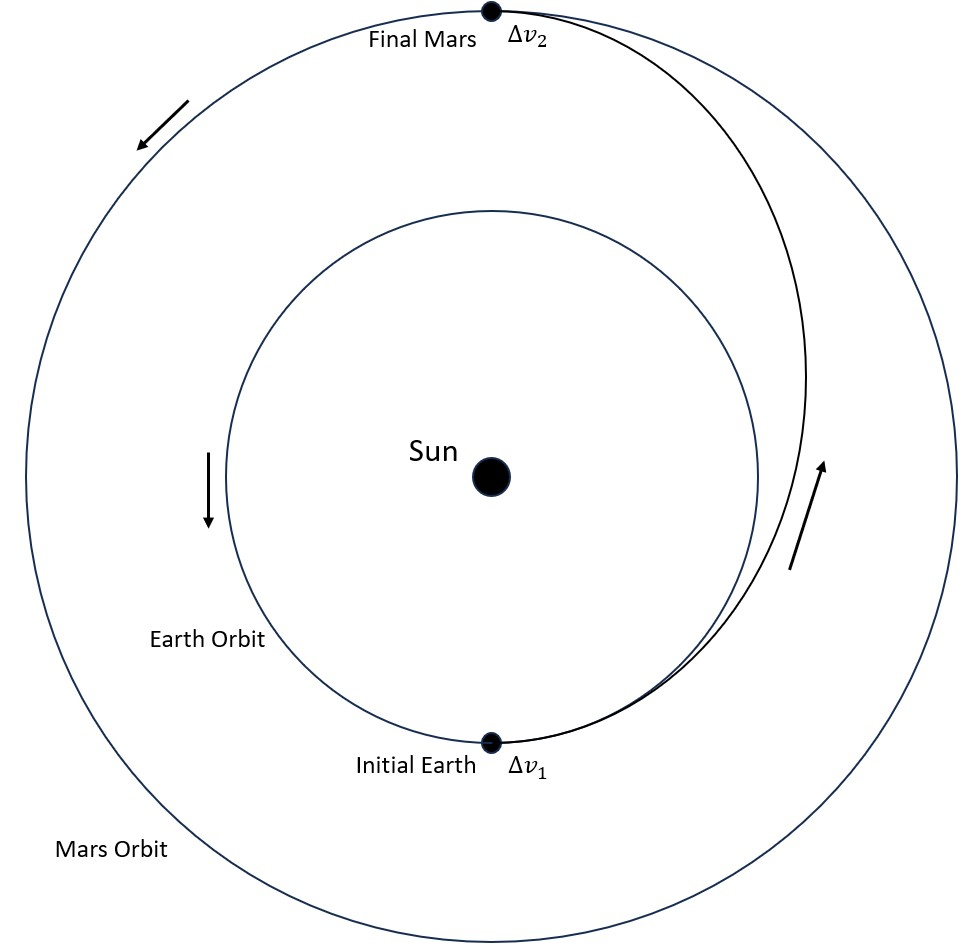
\includegraphics[width=0.5\textwidth]{figures/Hohmann.jpg}
    \caption{Hohmann transfer between Earth and Mars.}
    \label{fig:Hohmann}
\end{figure}

To serve as a baseline transfer between cislunar orbits and a Sun-Mars $L_{1}$ halo orbit for this
investigation, a Hohmann transfer between the Earth orbit (assumed circular at a radius of
$1.49598\times10^{8}$) and the Sun-Mars $L_{1}$ distance ($2.26858\times10^{8}$) is constructed.
The following equations are applied to calculate the modified Hohmann transfer with a plane change:
\begin{equation}
    \Delta v_{1}=\sqrt{\frac{\mu_{2BP}}{r_{1}}}(\sqrt{\frac{2r_{2}}{r_{1}+r_{2}}}-1),
    \label{eq:Hohmann1}
\end{equation}
\vspace{1mm}
\begin{equation}
    \Delta v_{2}=\sqrt{v_{H}^{2}+v_{2}^{2}-2v_{H}v_{2}\cos\Delta i},
    \label{eq:Hohmann2}
\end{equation}
\vspace{1mm}
\begin{equation}
    v_{H}=\sqrt{\frac{\mu_{2BP}}{r_{2}}(\frac{2r_{1}}{r_{1}+r_{2}})},
    \label{eq:transferv}
\end{equation}
\vspace{1mm}
\begin{equation}
    v_{2}=\sqrt{\frac{\mu_{2BP}}{r_{2}}},
    \label{eq:circlev}
\end{equation}
where $\Delta v_{1}$ and $\Delta v_{2}$ are the two burns of the transfer, $\mu_{2BP}$ is the
gravitational parameter of the Sun, $r_{1}$ and $r_{2}$ are the Earth orbit and Sun-Mars $L_{1}$
radii, respectively, $v_{H}$ is the velocity at apoapsis of the Hohmann transfer ellipse, $v_{2}$
is the circular velocity at Sun-Mars $L_{1}$, and $\Delta i$ is the difference in inclination
between the two orbital planes. The framework results in a total $\Delta v$ for the modified
Hohmann transfer of $5.639$ km/s, that is directly compared to the total maneuver costs of the two
categories of transfers developed in this investigation to find transfers with lower costs. Note
that the minimum $\Delta v$ required to reach the Sun-Mars $L_{1}$ radius from Earth orbit,
assuming that a maneuver-less strategy is implemented to decelerate upon arrival, is $2.914$ km/s.
The comparison highlights the potential for more efficient transfer strategies that reduce the
overall maneuver cost compared to a baseline modified Hohmann transfer, while also providing a
benchmark for evaluating the effectiveness of alternative approaches.

As stated previously, the modified Hohmann transfer performs the plane change maneuver at the
apoapsis of the transfer ellipse, implying that the lowest cost MMAT transfers occur when their
second burn is located at the apoapsis of the bridge conic arc. The TOF of the Hohmann transfer
arc is calculated analytically:
\begin{equation}
    TOF=\pi\sqrt{\frac{(r_{1}+r_{2})^{2}}{7\mu_{2BP}}},
    \label{eq:HohmannTOF}
\end{equation}
which is analogous to the times-of-flight of the MMAT bridge conic arcs. The minimum-$\Delta v$
transfer has a TOF of $258$ days. The time-of-flight serves as a reference point for evaluating the
temporal efficiency of MMAT bridge arcs relative to the modified Hohmann transfer.
